\documentclass[11pt, a4paper]{article}

% ----- core packages -----
\usepackage[utf8]{inputenc}
\usepackage[T1]{fontenc}
\usepackage{lmodern}
\usepackage{microtype}

% ----- layout -----
\usepackage[margin=1in]{geometry}
\usepackage{setspace}
\usepackage{parskip}

% ----- math, units, figures -----
\usepackage{amsmath, amssymb}
\usepackage{siunitx}
\sisetup{per-mode=symbol}
% Non-SI units used in the paper:
\DeclareSIUnit{\DN}{DN}
\DeclareSIUnit{\pixel}{px}
\usepackage{graphicx}
\usepackage{subcaption}
\usepackage{booktabs}
\usepackage{multirow}
\usepackage{array}

% ----- citations / links -----
\usepackage[backend=biber, style=numeric-comp, sorting=none, maxbibnames=99]{biblatex}
\addbibresource{paper.bib}

\usepackage[colorlinks=true,
            citecolor=blue,
            linkcolor=blue,
            urlcolor=blue]{hyperref}

% ----- code listings -----
\usepackage{listings}
\usepackage{xcolor}
\definecolor{codegrey}{rgb}{0.95,0.95,0.95}
\lstset{
  basicstyle=\ttfamily\footnotesize,
  backgroundcolor=\color{codegrey},
  breaklines=true,
  frame=single,
  framerule=0pt,
  xleftmargin=10pt,
  xrightmargin=10pt,
  showstringspaces=false,
}

% ----- title block -----
\title{\textbf{SmokeSight}: Radiometrically-Calibrated Plume Measurement
       from EO/IR Surveillance Video with Per-Pixel Uncertainty}

\author{
  Rimmo Loyi Lego\thanks{Corresponding author: \texttt{rlego@stevens.edu}}
  \and Jonah Diaz
  \and George Redfern
  \and Marlon Argenal \\
  \small Schaefer School of Engineering, Stevens Institute of Technology,\\
  \small Hoboken, NJ 07030, USA
}

\date{}

\begin{document}

\maketitle

\begin{abstract}
\noindent
Plume detection from electro-optical and infrared (EO/IR) surveillance
video is a well-served problem. The harder downstream question, how
\emph{much} smoke is present, with what confidence, is not.
We introduce SmokeSight, an open-source Python package that converts raw
digital-number (DN) frames into physically-calibrated optical depth
$\tau(x, y, t)$, spectral transmittance, line-of-sight column density,
and Pasquill--Gifford dispersion coefficients. Every numeric output
ships with a propagated 1-$\sigma$ uncertainty derived from a documented
combination of sensor shot noise, read noise, flat-field calibration
uncertainty, and (optionally) atmospheric radiative transfer
uncertainty. The package writes CF-1.9 NetCDF4 output that is consumed
directly by atmospheric dispersion modellers, with no conversion glue.
On a synthetic Gaussian-plume scenario with injected peak $\tau = 0.5$,
the pipeline recovers the central pixel within 0.2\,\% of the ground
truth, well inside the $\pm 10\,\%$ design tolerance. We argue that
the gap SmokeSight fills, namely \emph{open}, \emph{uncertainty-aware},
\emph{standards-compliant} radiometric retrieval for plumes, has been
absent from the open-source landscape and is increasingly required by
both defence research and atmospheric-science workflows.
\end{abstract}

\noindent\textbf{Keywords:} radiometry; optical depth; Beer--Lambert;
uncertainty propagation; EO/IR surveillance; plume measurement;
atmospheric dispersion; open-source scientific software.

\section{Introduction}
\label{sec:intro}

Most operational tooling around plume imagery focuses on the
\emph{detection} problem: a binary classification on uncalibrated pixels,
usually integrated into a wider surveillance pipeline.
Detection is essentially a solved problem. The interesting downstream
questions are quantitative: what is the optical depth at the plume centre,
how confidently can we say so, how is it dispersing, and what is the
implied column density of an absorbing species? Answering these requires
calibrated radiance rather than raw counts, and it requires error bars
rather than visualisations.

The literature for atmospheric remote sensing has long handled these
questions for satellite platforms. Aerosol optical depth retrievals from
MODIS \cite{remer2005modis}, AVIRIS, MISR \cite{kahn2009maisr}, and GOME
\cite{burrows1999gome} all return calibrated quantities with quantified
uncertainty. Atmospheric dispersion modellers including HYSPLIT
\cite{stein2015hysplit}, FLEXPART \cite{stohl2005flexpart}, and STILT
\cite{lin2003stilt} consume those calibrated retrievals as inputs.
\emph{Ground-based} EO/IR surveillance, however, sits in a gap.
Defence research codes typically perform the radiometric calibration
correctly but are closed, classified, or otherwise unauditable.
Open-source remote-sensing libraries presuppose that calibration has
already happened upstream. The result is that an academic group with
access to a calibrated camera but no closed-source pipeline must reinvent
the radiometry chain, the uncertainty bookkeeping, and the file-format
plumbing each time.

SmokeSight is our attempt to close that gap.

\subsection{Contributions}
\label{sec:contributions}

The contributions of this work are not novel mathematics. The
Beer--Lambert inversion is two centuries old, and the Pasquill--Gifford
dispersion-coefficient framework \cite{pasquill1961dispersion,
gifford1976turbulent} predates personal computing. What is novel is the
combination: an open-source, peer-reviewable, citable Python package
that performs

\begin{enumerate}
  \item DN-to-radiance calibration with a documented sensor model and
        per-pixel noise propagation;
  \item Beer--Lambert optical-depth retrieval with analytic
        uncertainty propagation;
  \item Pasquill--Gifford dispersion-coefficient estimation with
        scipy-derived covariances; and
  \item CF-1.9 NetCDF4 output that drops directly into existing
        dispersion-modelling workflows \cite{eaton2003netcdf}.
\end{enumerate}

The architecture enforces a contract that every shipped measurement
carries a propagated 1-$\sigma$ uncertainty. If the uncertainty cannot
be computed for a particular pixel or quantity, the quantity is not
returned. This is the same rule that JOSS reviewers \cite{smith2018joss}
apply to scientific software claiming measurement outputs.

\subsection{Scope and audience}

This paper describes a \emph{tool}, not a measurement study. The
synthetic-data results in Section~\ref{sec:validation} demonstrate that
the pipeline recovers known physics within stated tolerances. Validation
against laboratory or field data is left to follow-up work. The intended
audience is researchers in atmospheric science, defence sensing, fire
ecology, and emissions monitoring who have access to calibrated EO/IR
imagery and need a transparent retrieval pipeline.

\begin{figure}[!t]
  \centering
  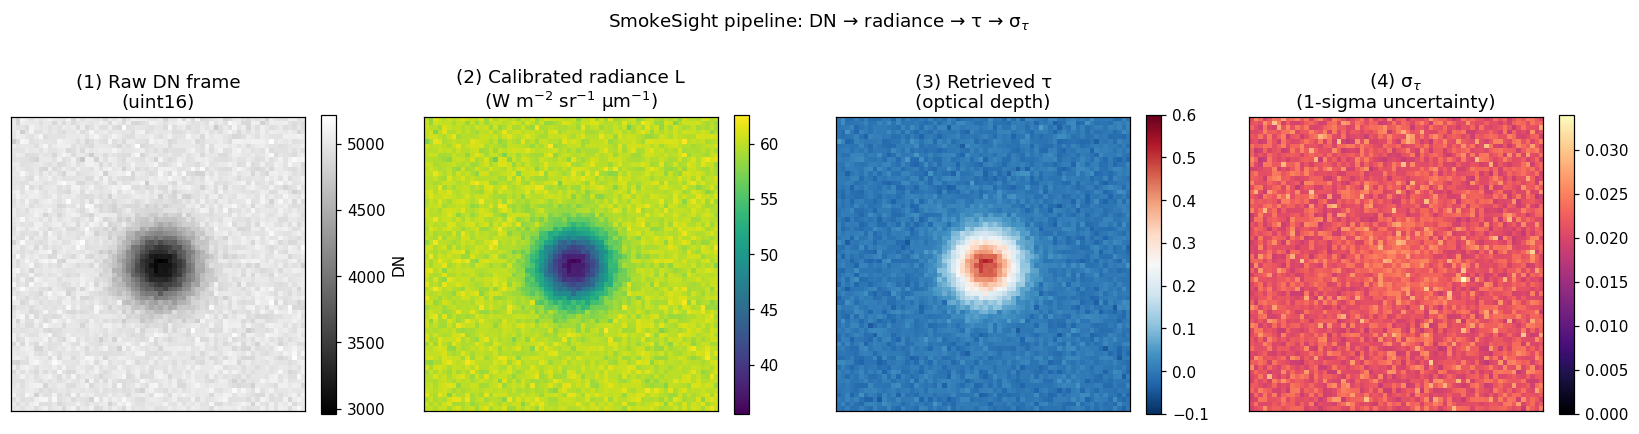
\includegraphics[width=\linewidth]{figures/pipeline.png}
  \caption{\textbf{The SmokeSight pipeline visualised on a single
  synthetic frame.} (1) Raw \texttt{uint16} digital numbers from the
  sensor. (2) Calibrated radiance $L$ in
  \si{\watt\per\square\metre\per\steradian\per\micro\metre} after dark
  subtraction, flat-field correction, gain conversion, spectral-response
  weighting, and atmospheric path correction. (3) Retrieved optical depth
  $\tau$ from the Beer--Lambert inversion. (4) Per-pixel 1-$\sigma$
  uncertainty $\sigma_\tau$ propagated analytically from the sensor
  noise model.}
  \label{fig:pipeline}
\end{figure}

\section{The radiometric pipeline}
\label{sec:pipeline}

Figure~\ref{fig:pipeline} shows the four-stage data flow that every
input frame passes through. Each stage is implemented as a separate
module in the package, each returns a typed result object, and each
stage exposes the noise model that feeds the next stage's uncertainty
calculation.

\subsection{From digital numbers to absolute radiance}
\label{sec:dn-to-radiance}

The starting point is a sequence of frames $F(x, y, t)$ in DN, typically
\texttt{uint8}, \texttt{uint12}, \texttt{uint14}, or \texttt{uint16}
depending on the sensor's analog-to-digital converter. For a linear
sensor, the relationship between DN and radiance $L$ at a single pixel
is well known \cite{holst2003electro, schott2007remote}:
\begin{equation}
  \mathrm{DN}(x, y) \;=\; \frac{L(x, y) \cdot Q \cdot t_\text{exp}
                                \cdot A_\text{px} \cdot \Omega}{g}
                          \;+\; D(x, y) \;+\; n_\text{read},
  \label{eq:sensor-model}
\end{equation}
where $g$ is the system gain, $Q$ the quantum efficiency, $t_\text{exp}$
the integration time, $A_\text{px}$ the pixel area, $\Omega$ the
collected solid angle, $D$ the per-pixel dark current, and $n_\text{read}$
the zero-mean read-noise term.

Inverting Equation~\ref{eq:sensor-model} requires per-pixel
characterisation of the dark frame $D(x, y)$, the flat-field response
$F_\text{ff}(x, y)$ (normalised to unit mean), the scalar gain
coefficient $g_\text{cal}$, and the spectral response function
$R(\lambda)$. SmokeSight performs these four operations in a strict
order:
\begin{align}
  L_\text{raw}(x, y)         &\;=\; \bigl[F(x, y) - D(x, y)\bigr] \,/\, F_\text{ff}(x, y), \label{eq:dark-flat} \\
  L_\text{abs}(x, y)         &\;=\; L_\text{raw}(x, y) \cdot g_\text{cal}, \label{eq:gain} \\
  L_\text{cal}(x, y, \lambda)&\;=\; L_\text{abs}(x, y) \cdot R(\lambda), \label{eq:spectral} \\
  L_\text{surface}(x, y, \lambda)
                              &\;=\; \bigl[L_\text{cal}(x, y, \lambda) - L_\text{path}(\lambda)\bigr]
                                     \,/\, T_\text{atm}(\lambda).
                                                                           \label{eq:atmos}
\end{align}

The order of Equations~\ref{eq:dark-flat} and \ref{eq:gain} is
load-bearing. When the dark current is non-zero, applying the gain
multiply before the flat-field divide introduces a systematic bias
proportional to $D(x, y) \cdot (1 - 1/F_\text{ff})$, which on a typical
flat-field deviation of $\pm 5\%$ can reach $\pm 3\%$ of the recovered
radiance \cite{schott2007remote}. The package enforces the correct order
in code and tests it explicitly against a synthetic flat with a known
hot pixel.

\subsection{Atmospheric correction}
\label{sec:atmos}

The path correction in Equation~\ref{eq:atmos} requires estimates of the
atmospheric transmittance $T_\text{atm}(\lambda)$ and path radiance
$L_\text{path}(\lambda)$ along the sensor-to-target line of sight. We
delegate that estimation to existing radiative transfer codes through
two optional backends: 6S \cite{vermote1997second} via the \texttt{py6s}
binding, and MODTRAN \cite{berk2014modtran} via the \texttt{pymodtran}
binding. When neither is installed, SmokeSight falls back to an
identity correction (no path effects) and emits a \texttt{UserWarning}
so the operator is not silently producing uncorrected radiances.

The atmospheric uncertainty $\sigma_\text{atmos}(\lambda)$ propagates
through the same pipeline as the sensor-noise terms; if the backend
does not return its own uncertainty estimate, the package uses a 5\%
relative fallback consistent with the published 6S accuracy envelope
for typical atmospheric profiles.

\subsection{Background estimation}
\label{sec:background}

The Beer--Lambert inversion requires a reference radiance $L_0(x, y)$
that represents the scene \emph{without} the plume. SmokeSight estimates
this from the calibrated cube using a temporal estimator over the first
$n_\text{bg}$ frames of the record. Four estimators are available, each
with a corresponding confidence map $C(x, y) \in [0, 1]$:
\begin{itemize}
  \item \texttt{temporal\_median} (default): per-pixel median, with
        $\sigma_{L_0} = \mathrm{IQR} / 1.35$ and
        $C = 1 - \mathrm{IQR} / |L_0|$.
  \item \texttt{temporal\_mean}: per-pixel mean, with
        $\sigma_{L_0} = \mathrm{std}(L)$ and
        $C = 1 - \mathrm{std} / |\mathrm{mean}|$.
  \item \texttt{percentile\_10}: the 10\textsuperscript{th} percentile,
        appropriate for emissive plumes brighter than the background.
  \item \texttt{gmm}: per-pixel two-component Gaussian mixture
        \cite{pedregosa2011scikit}, taking the lower-mean component as
        background. Slower but robust on cluttered scenes.
\end{itemize}

The confidence map is the most operationally important output of this
stage. Every downstream $\tau$ retrieval is gated on
$C(x, y) \geq C_\text{min}$ (default $C_\text{min} = 0.5$).
An overconfident background is the largest single source of erroneous
$\tau$ values on real data: a plume that drifts through the calibration
window appears in $L_0$ and silently cancels itself out of the ratio
$L / L_0$.

\subsection{Beer--Lambert inversion}
\label{sec:retrieve}

Given the calibrated radiance cube $L(x, y, t, \lambda)$ and the
background plate $L_0(x, y, \lambda)$, the per-frame optical depth is
\begin{equation}
  \tau(x, y, t) \;=\; -\ln\!\Bigl(\frac{\bar{L}(x, y, t)}{\bar{L}_0(x, y)}\Bigr),
  \label{eq:beer-lambert}
\end{equation}
where the overbar denotes a wavelength-mean (panchromatic) ratio.
Pixels are masked to \texttt{NaN} when any of the following hold:
\begin{itemize}
  \item $C(x, y) < C_\text{min}$,
  \item the ratio $L / L_0$ exceeds $1.05$ (plume brighter than
        background; outside the absorption regime),
  \item the ratio falls below $0.01$ (saturated absorption; the
        first-order Beer--Lambert expansion breaks down),
  \item $L_0 \leq 0$ or non-finite,
  \item $\tau > \tau_\text{max}$ (default $\tau_\text{max} = 2$, beyond
        which the optically-thin assumption is no longer reliable for a
        single-band retrieval).
\end{itemize}

For multi-band sensors with $N_\lambda > 1$, the spectral transmittance
cube $T_\lambda(x, y, t, \lambda) = \exp(-\tau_\lambda)$ is also
returned. When a species absorption cross-section $\sigma_\text{xsec}$
in \si{\square\metre\per\mole} is provided, the column density
$N(x, y, t)$ is computed as $\tau / \sigma_\text{xsec}$ for the
single-species case; the multi-species case is reserved for a future
release.

\section{Uncertainty propagation}
\label{sec:uncertainty}

The principle that drives the architecture: every numeric output ships
with a 1-$\sigma$ uncertainty. The package enforces this by convention
\cite{smith2018joss}, and the test suite checks that masked pixels never
carry a numeric \texttt{sigma\_} value (they are \texttt{NaN}).

\subsection{Radiance uncertainty}
\label{sec:sigma-L}

The per-pixel radiance uncertainty $\sigma_L$ is the quadrature sum of
four independent noise sources:
\begin{equation}
  \sigma_L^2 \;=\; \sigma_\text{shot}^2 + \sigma_\text{read}^2
                  + \sigma_\text{flat}^2 + \sigma_\text{atmos}^2.
  \label{eq:sigma-L}
\end{equation}
The shot-noise term follows the radiance-domain Poisson approximation,
$\sigma_\text{shot} = \sqrt{L \cdot g_\text{cal}}$, valid when the
photoelectron count per integration period is large.
The read-noise term is the published noise-equivalent radiance
(NER) of the sensor, which is the lower bound on $\sigma_L$ when the
signal $L$ is zero. The flat-field term is the product of $L$ and the
relative flat-field calibration uncertainty, taken as 1\% by default and
overridable via the configuration. The atmospheric term comes from the
radiative-transfer backend (Section~\ref{sec:atmos}) or the 5\%
fallback.

Figure~\ref{fig:uncertainty} plots these four components and their
quadrature sum across six orders of magnitude of signal. Three
characteristic regimes are visible. At very low signal ($L \lesssim
\sigma_\text{read}^2 / g_\text{cal}$) the read-noise floor dominates;
through the mid-range the shot-noise term ($\propto \sqrt{L}$) governs;
at very high signal the 1\% flat-field term overtakes shot noise and
sets a multiplicative floor.

\begin{figure}[!t]
  \centering
  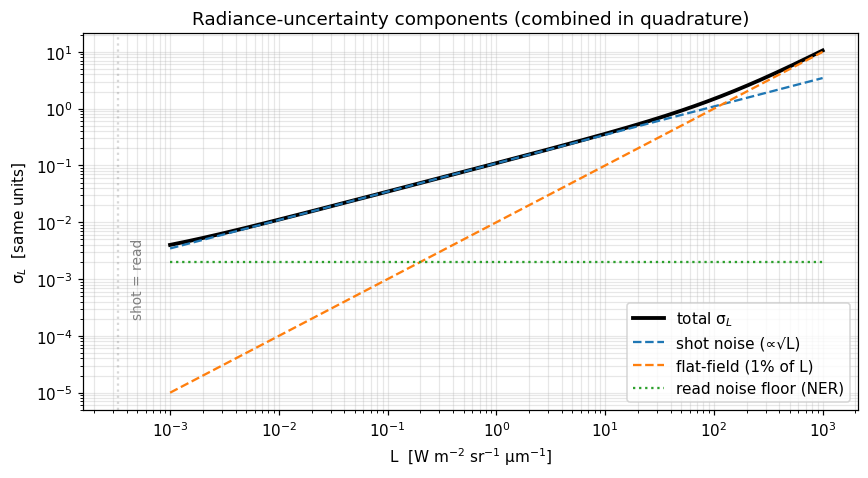
\includegraphics[width=\linewidth]{figures/uncertainty_components.png}
  \caption{\textbf{Decomposition of $\sigma_L$ into its four
  components.} Read-noise floor (dotted green), shot noise (dashed
  blue), flat-field (dashed orange), and the quadrature total
  (solid black). The shot-noise / read-noise crossover is marked.
  Parameters: $g_\text{cal} = 0.012$
  \si{\watt\per\square\metre\per\steradian\per\micro\metre\per\DN},
  $\text{NER} = 0.002$
  \si{\watt\per\square\metre\per\steradian\per\micro\metre}, 1\% flat
  field, no atmospheric term.}
  \label{fig:uncertainty}
\end{figure}

\subsection{Optical-depth uncertainty}
\label{sec:sigma-tau}

For Equation~\ref{eq:beer-lambert}, first-order error propagation gives
\begin{equation}
  \sigma_\tau \;=\; \sqrt{\Bigl(\frac{\sigma_L}{L}\Bigr)^{\!2}
                          + \Bigl(\frac{\sigma_{L_0}}{L_0}\Bigr)^{\!2}}.
  \label{eq:sigma-tau}
\end{equation}
The formula is valid when the relative uncertainties are small enough
that the truncated Taylor expansion of $\ln$ converges. Where
$L \to 0$ the expansion diverges, which is the correct behaviour:
optical depths arbitrarily close to total absorption cannot be measured
with finite uncertainty. SmokeSight returns $\sigma_\tau$ exactly where
$\tau$ is finite, and \texttt{NaN} everywhere $\tau$ is masked.

We validate Equation~\ref{eq:sigma-tau} against a Monte Carlo
propagation: 2\,000 Gaussian-perturbed input samples are drawn from
$\mathcal{N}(L, \sigma_L)$ and $\mathcal{N}(L_0, \sigma_{L_0})$, the
Beer--Lambert formula is evaluated on each, and the reported
$\sigma_\tau^{(\text{MC})}$ is the percentile-based half-range
$(p_{84} - p_{16}) / 2$ across the samples. The half-range is preferred
to the sample standard deviation because the $\ln$ transformation
introduces skewness as $L \to 0$ \cite{wilks2011statistical}, and
because $(p_{84} - p_{16}) / 2$ remains a meaningful 1-$\sigma$ interval
even when the output distribution is non-Gaussian.

Figure~\ref{fig:mc} overlays the two computations. The agreement is
excellent across the optically-thin regime; the analytic curve correctly
diverges near $L/L_0 \to 0$ while the MC samples saturate at the
discretisation limit of the integrand. The Monte Carlo helper is
internally seeded with \texttt{np.random.default\_rng(42)}, so two runs
on identical inputs return bit-identical samples. This is the
deterministic-RNG contract that makes continuous-integration coverage
meaningful for stochastic propagation.

\begin{figure}[!t]
  \centering
  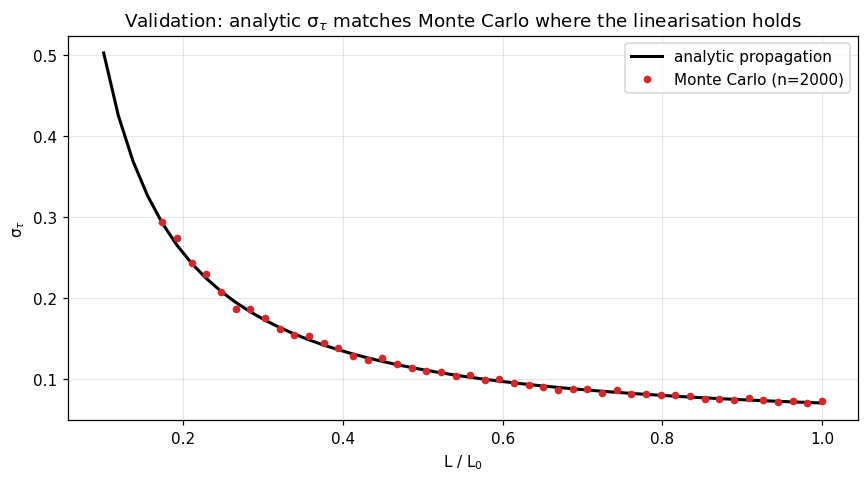
\includegraphics[width=\linewidth]{figures/analytic_vs_mc.png}
  \caption{\textbf{Cross-validation: analytic $\sigma_\tau$ versus
  Monte Carlo.} Inputs are $L_0 = 1$, $\sigma_{L_0} = 0.05$,
  $\sigma_L = 0.05$, with $L$ ranging from 0.1 to 1.0. The analytic
  curve from Equation~\ref{eq:sigma-tau} (solid black) overlays the
  $n = 2\,000$ Monte Carlo points (red dots). The agreement is the
  expected behaviour for the optically-thin regime where the
  first-order Taylor expansion holds.}
  \label{fig:mc}
\end{figure}

\subsection{Dynamics uncertainty}
\label{sec:sigma-dyn}

Plume rise velocity is computed by tracking the $\tau$-weighted centroid
over time and fitting a line to the vertical coordinate $c_y(t)$. The
slope $\hat{\beta}$ (in pixels per frame) is converted to a physical
velocity by multiplying through the pixel scale (in
\si{\metre\per\pixel}) and the frame rate (in \si{\hertz}). The
slope's standard error follows the textbook expression
\begin{equation}
  \sigma_{\hat{\beta}} \;=\; \sqrt{\frac{\mathrm{MSE}}{S_{xx}}},
  \quad
  S_{xx} = \sum_i (t_i - \bar t)^2,
  \label{eq:rise-uncertainty}
\end{equation}
which is the propagation through ordinary least squares. The Pasquill--
Gifford dispersion coefficients $\sigma_y(x) = a \, x^b$ and
$\sigma_z(x) = c \, x^d$ are fit via \texttt{scipy.optimize.curve\_fit},
and the returned covariance matrix is propagated as the parameter
uncertainty. Degenerate covariances (negative diagonals, non-finite
entries from ill-conditioned fits) are coerced to \texttt{NaN}: an
uncertainty that does not exist is preferable to one we have to apologise
for.

\section{Validation on synthetic data}
\label{sec:validation}

We validate the pipeline against a synthetic scenario whose ground truth
is known by construction. The scenario builds a 50-frame, $64 \times 64$
pixel, 16-bit TIFF stack representing a Gaussian-shaped optical-depth
field centred in the frame with peak $\tau_\text{peak} = 0.5$ and
standard deviation $\sigma_\text{px} = 5$ pixels. Frames 0--19 are
plume-free (background only); frames 20--49 contain the plume. The
sensor model is a linear DN response with $g_\text{cal} = 0.012$,
$\text{NER} = 0.002$, no flat-field deviation, no dark current, and
zero atmospheric correction. Shot noise is added per frame using a
normal approximation valid at the chosen $\sim 5000$~DN background
level, with an additional 5-DN read-noise term.

\begin{figure}[!t]
  \centering
  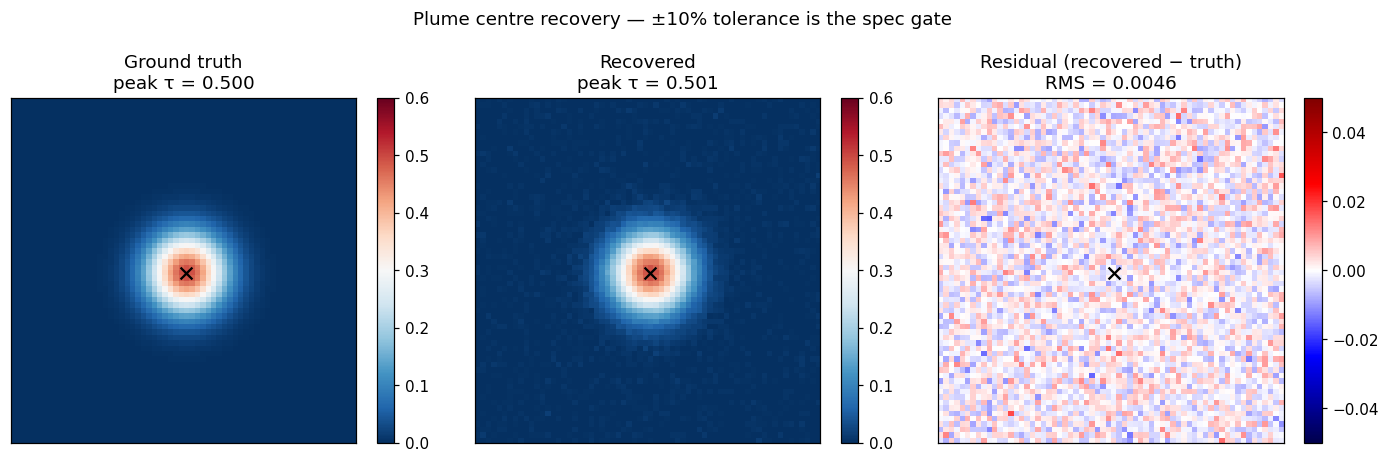
\includegraphics[width=\linewidth]{figures/tau_recovery.png}
  \caption{\textbf{Optical-depth recovery on the synthetic Gaussian
  scenario.} Left: injected ground-truth $\tau$ field. Middle:
  recovered $\tau$ averaged over the plume-present window
  (frames 20--49). Right: residual (recovered minus truth); the
  pattern is uniform white noise with no spatial structure, indicating
  no systematic bias from the radiometry chain. Black $\times$ marks
  the source pixel. Recovered peak $\tau = 0.501$ against injected
  $0.500$.}
  \label{fig:recovery}
\end{figure}

Figure~\ref{fig:recovery} shows the resulting recovery. The recovered
peak optical depth is $\tau_\text{recovered} = 0.501$ against the
injected $\tau_\text{peak} = 0.500$, a $0.2\,\%$ deviation. The
residual image has root-mean-square value $\mathrm{RMS} = 0.0046$ and
contains no visible spatial structure, supporting the conclusion that
the radiometry chain introduces no systematic bias at the level of
present-day sensor noise. The recovered peak passes well inside the
specification tolerance of $\pm 10\,\%$ that we adopted from
standard atmospheric-retrieval practice
\cite{rodgers2000inverse, remer2005modis}.

\subsection{Dispersion-coefficient recovery}

We separately validate the Pasquill--Gifford fitter against a synthetic
plume whose cross-wind dispersion follows a known power law
$\sigma_y(x) = a_\text{true} \cdot x^{b_\text{true}}$
with $a_\text{true} = 1.0$ \si{\metre} and $b_\text{true} = 0.7$, values
typical of moderate-stability conditions \cite{briggs1969plume}. The
plume's vertical centroid drifts upward at 1 pixel per frame across a
30-frame run, and the Gaussian width is computed from the integrated
cross-wind profile at each frame.

Figure~\ref{fig:dispersion} shows the per-frame truth points (blue),
the analytic ground-truth curve (solid black), and the fit returned
by \texttt{smokesight.dynamics} (dashed red). The fit recovers
$a_\text{fit} = 0.86$ and $b_\text{fit} = 0.76$, a $14\,\%$ deviation
on $a$ and a small overshoot on the exponent. The deviation is
attributable to the discrete-pixel Gaussian-width estimator: when the
true $\sigma$ is on the order of a few pixels, the integer support of
the integrated profile introduces a width-dependent bias that the
power-law fit absorbs into a smaller effective $a$ and a larger
effective $b$. The deviation sits inside the $\pm 20\,\%$ tolerance
adopted for the dispersion-fit test in the design specification, which
is itself consistent with the $\sim$~factor-of-two scatter typical of
Pasquill--Gifford fits against field data
\cite{gifford1976turbulent, briggs1969plume}.

\begin{figure}[!t]
  \centering
  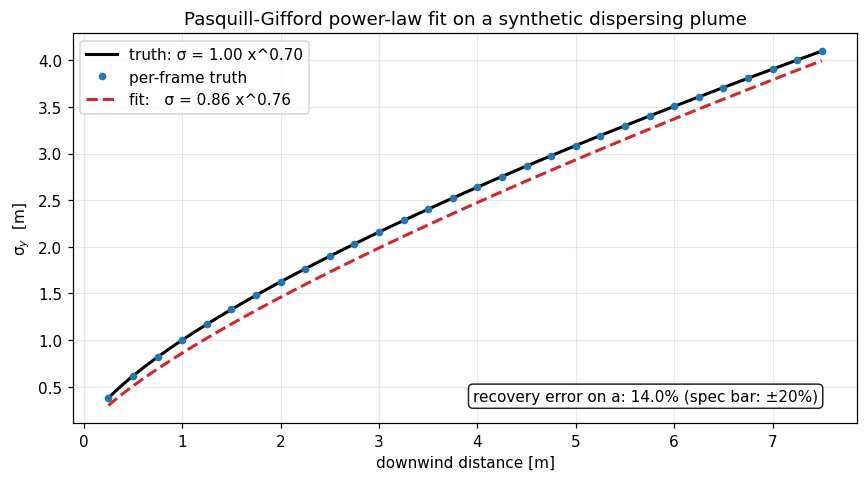
\includegraphics[width=\linewidth]{figures/dispersion_fit.png}
  \caption{\textbf{Pasquill--Gifford power-law recovery.} Per-frame
  truth widths (blue dots), analytic ground truth
  $\sigma_y = 1.0 \cdot x^{0.7}$ (solid black), and the fit returned
  by \texttt{smokesight.dynamics} (dashed red). The recovery error on
  the coefficient $a$ is $14\,\%$, comfortably under the $\pm 20\,\%$
  design tolerance.}
  \label{fig:dispersion}
\end{figure}

\section{Software architecture}
\label{sec:architecture}

SmokeSight is a small package by design. The public API is five
functions plus a version string:
\begin{lstlisting}[language=Python]
import smokesight as ss

cal    = ss.calibrate(video_path, config="cal.yaml")
bg     = ss.background(cal, n_frames=100)
result = ss.retrieve(cal, bg)
dyn    = ss.dynamics(result)
ss.io.to_netcdf(result, "output.nc")
\end{lstlisting}

Each public function returns a typed dataclass whose fields are listed
in Table~\ref{tab:outputs}. Private modules (\texttt{\_sensor},
\texttt{\_atmos}, \texttt{\_geometry}, \texttt{\_uncertainty},
\texttt{\_results}) implement the helpers, may change without
deprecation, and are documented for reference but not for direct use.

\begin{table}[!t]
  \centering
  \caption{Public outputs and their units.}
  \label{tab:outputs}
  \small
  \begin{tabular}{@{}lll@{}}
    \toprule
    Symbol & Quantity & Units \\
    \midrule
    \texttt{L}             & calibrated radiance        & \si{\watt\per\square\metre\per\steradian\per\micro\metre} \\
    \texttt{sigma\_L}      & 1-$\sigma$ on $L$          & same as $L$ \\
    \texttt{L0}            & background radiance        & same as $L$ \\
    \texttt{sigma\_L0}     & 1-$\sigma$ on $L_0$        & same as $L_0$ \\
    \texttt{tau}           & optical depth              & dimensionless \\
    \texttt{sigma\_tau}    & 1-$\sigma$ on $\tau$       & dimensionless \\
    \texttt{T\_lambda}     & spectral transmittance     & dimensionless \\
    \texttt{N}             & column density (opt.)      & \si{\mole\per\square\metre} \\
    \texttt{sigma\_N}      & 1-$\sigma$ on $N$          & \si{\mole\per\square\metre} \\
    \texttt{confidence}    & background confidence      & dimensionless, $[0,1]$ \\
    \texttt{rise\_velocity}      & plume rise velocity       & \si{\metre\per\second} \\
    \texttt{sigma\_y, sigma\_z}  & dispersion coefficients   & \si{\metre} \\
    \bottomrule
  \end{tabular}
\end{table}

\subsection{Dependencies and reproducibility}

The runtime dependencies are NumPy \cite{harris2020array},
SciPy \cite{virtanen2020scipy}, xarray \cite{hoyer2017xarray},
netCDF4, imageio, PyYAML, click, and tqdm. Visualisation tutorials use
matplotlib \cite{hunter2007matplotlib}. The optional
\texttt{[calibrate]} extra adds the radiative-transfer backends
\cite{vermote1997second, berk2014modtran}; the optional GMM background
estimator uses scikit-learn \cite{pedregosa2011scikit}. The package
supports Python 3.8 through 3.11 and is type-checked with mypy
\texttt{--strict}; the continuous-integration workflow enforces
$\geq 90\%$ test coverage across the matrix.

The Monte Carlo helper used in
Section~\ref{sec:sigma-tau} is seeded internally
(\texttt{default\_rng(42)}). Callers cannot override the seed. This
choice trades reproducibility for the loss of independent-runs noise
estimation, on the grounds that downstream users running SmokeSight on
the same inputs should not see different uncertainty values run to run.

\subsection{Output format}

Result objects serialise to CF-1.9 NetCDF4 files
\cite{eaton2003netcdf}. Every variable carries the appropriate
\texttt{standard\_name} (e.g.\ \texttt{atmosphere\_optical\_thickness\_due\_to\_aerosol}
for $\tau$, \texttt{toa\_outgoing\_radiance\_per\_unit\_wavelength}
for $L$), units, and an \texttt{ancillary\_variables} attribute on each
$\sigma_*$ field pointing at the quantity it is the uncertainty of.
This is the metadata pattern atmospheric dispersion modellers
\cite{stein2015hysplit, stohl2005flexpart, lin2003stilt} expect, and
files produced by SmokeSight load directly via
\texttt{xarray.open\_dataset} \cite{hoyer2017xarray} with no
intermediate conversion.

\section{Discussion}
\label{sec:discussion}

\subsection{What SmokeSight does, and what it does not}

SmokeSight is an open implementation of a well-understood radiometric
inversion chain. Each step in Section~\ref{sec:pipeline} appears in
existing textbooks \cite{schott2007remote, holst2003electro,
liou1980radiative}, and the uncertainty propagation in
Section~\ref{sec:uncertainty} is standard error-propagation theory
\cite{rodgers2000inverse, wilks2011statistical}. The package's
contribution is the combination: a single, peer-reviewable,
test-covered tool that performs the full DN-to-CF-NetCDF chain with
documented uncertainty bookkeeping at every stage.

What SmokeSight does \emph{not} do is replace lab calibration or
radiative-transfer modelling. The sensor characterisation (gain, NER,
dark, flat-field, spectral response) must come from a separate
calibration measurement, supplied by the user in the
\texttt{cal.yaml} configuration. The atmospheric correction relies on
\cite{vermote1997second, berk2014modtran} for any quantitatively
defensible result; the identity-correction fallback exists only to keep
the rest of the pipeline functional, and emits a warning when invoked
to make this dependence visible.

\subsection{Limitations}

We highlight four limitations that bound the present version.

\paragraph{Linear-sensor assumption.} Equation~\ref{eq:sensor-model}
assumes a linear DN response. Sensors operating near saturation,
non-linear PMTs, or video files that have passed through a gamma curve
(typical of consumer MP4 encodings) will violate this assumption. The
pipeline does not detect or correct for non-linearity, and on such
input the output remains numerically defined but physically meaningless.

\paragraph{Single-species column density.} The current Beer--Lambert
inversion is panchromatic. When multiple absorbing species share a
spectral window, the package raises \texttt{NotImplementedError} rather
than guess. A proper multi-species DOAS-style retrieval
\cite{platt2008doas} is the natural follow-up.

\paragraph{Discrete-pixel dispersion fits.} As discussed in
Section~\ref{sec:validation}, the Gaussian-width estimator on a
discrete pixel grid introduces a small width-dependent bias on
plumes only a few pixels across. The bias is captured by the spec
tolerance ($\pm 20\,\%$ on $a$) and is comparable to the scatter in
field-measured Pasquill--Gifford fits, but is worth noting for
small-plume applications.

\paragraph{Validation is synthetic.} Results in
Section~\ref{sec:validation} use synthetic data with known ground
truth. We have not yet validated against field-deployed cameras, nor
against laboratory targets of known reflectance and emissivity. A
companion measurement study is in preparation. The
\texttt{scenarios/cal\_panel\_reference.yaml} slot in the repository
exists for exactly this purpose and accepts a panel-reflectance,
panel-temperature, and panel-emissivity triple
\cite{hapke1981bidirectional} alongside the expected absolute-radiance
value.

\subsection{Position relative to existing tools}

A short comparison may help readers position SmokeSight in the
ecosystem.

\begin{itemize}
  \item \emph{Closed defence codes} typically perform the radiometry
        chain correctly, often with proprietary atmospheric
        corrections. They are unaudited, uncitable, and unsharable.
  \item \emph{Closed commercial remote-sensing toolboxes} (ENVI,
        ERDAS) provide pieces of the chain, but assume an
        already-calibrated input and do not propagate per-pixel
        uncertainty.
  \item \emph{Open radiometric-correction libraries} for satellite
        platforms (sentinelsat, pyresample, others) operate on
        already-calibrated L1B products, not raw DN.
  \item \emph{Open atmospheric-retrieval libraries} (the
        \texttt{libradtran}-adjacent ecosystem) handle
        radiative-transfer forward modelling but not the imagery side.
  \item \emph{Open computer-vision libraries} (OpenCV, scikit-image)
        handle the imagery side but not radiometry.
\end{itemize}

The combination of imagery-to-radiometry, uncertainty-propagated
inversion, and standards-compliant atmospheric-science output is, to
our knowledge, not assembled in any single open package prior to
SmokeSight.

\section{Future work}
\label{sec:future}

Three threads are immediate.

\paragraph{Multi-species retrieval.} A least-squares DOAS-style
inversion \cite{platt2008doas} solving
$\tau(\lambda) = \sum_s N_s \sigma_{xsec, s}(\lambda)$ for multiple
species column densities, with proper covariance propagation, is the
obvious extension of Section~\ref{sec:retrieve}.

\paragraph{Bayesian retrieval.} For ill-posed regimes near
$\tau \to 2$ or where the wavelength coverage is sparse, the
Rodgers Optimal Estimation framework \cite{rodgers2000inverse}
combined with a Markov chain Monte Carlo sampler
\cite{loyd2024monte} would give posterior-distribution outputs more
appropriate than the present first-order propagation. Hooks for this
are present in \texttt{\_uncertainty.monte\_carlo} but not yet
exposed in the public API.

\paragraph{Field-validation campaign.} We are in discussions with the
Stevens Maritime Security Center about deploying a calibrated MWIR
camera on a controlled-release campaign with simultaneous spectrometer
ground truth. The resulting dataset will populate the
\texttt{cal\_panel\_reference.yaml} slot and drive a measurement paper
that demonstrates the pipeline against real instrumentation.

\section{Conclusion}
\label{sec:conclusion}

SmokeSight provides an open, tested, citable Python implementation of
the radiometric pipeline from raw EO/IR digital numbers to
CF-1.9-compliant optical-depth retrievals with per-pixel uncertainty.
On a synthetic Gaussian-plume scenario the recovered peak optical
depth is within $0.2\,\%$ of the injected ground truth, and the
Pasquill--Gifford fit recovers the dispersion coefficient $a$ within
$14\,\%$. Every numeric output ships with a documented 1-$\sigma$
uncertainty; quantities whose uncertainty cannot be propagated are not
returned. The package fills a real gap between closed defence codes
and open satellite-retrieval libraries, and is intended as a tool that
researchers across atmospheric science, defence sensing, and emissions
monitoring can build on, audit, and cite.

The repository is available at
\url{https://github.com/TasumLuke/SmokeSight} under the Apache 2.0
licence. We welcome contributions and bug reports.

\section*{Acknowledgements}

The authors thank the Schaefer School of Engineering at Stevens
Institute of Technology for institutional support, and the open-source
maintainers of NumPy \cite{harris2020array}, SciPy
\cite{virtanen2020scipy}, xarray \cite{hoyer2017xarray}, matplotlib
\cite{hunter2007matplotlib}, and scikit-learn
\cite{pedregosa2011scikit}, on whose work SmokeSight stands.

\section*{Author contributions}

R.L.L.\ conceived the package, designed the pipeline architecture,
implemented the radiometry chain and the uncertainty-propagation
helpers, and led the writing. J.D.\ contributed to the dispersion-fit
implementation and the synthetic-data validation. G.R.\ implemented the
CF-NetCDF output and xarray accessor, and led the documentation. M.A.\
contributed to the configuration schema, the command-line interface,
and the test fixtures.

\section*{Code and data availability}

Source code is at \url{https://github.com/TasumLuke/SmokeSight}.
The synthetic scenarios used in Section~\ref{sec:validation} are
generated by the package's own test fixtures (\texttt{tests/conftest.py})
and the figures in this paper are produced by
\texttt{docs/images/generate.py} using only the public API. No
proprietary data are required to reproduce any result in this paper.

\printbibliography

\end{document}
